\section{Conjunto de Dados}

\begin{figure}[!ht]
  \centering
  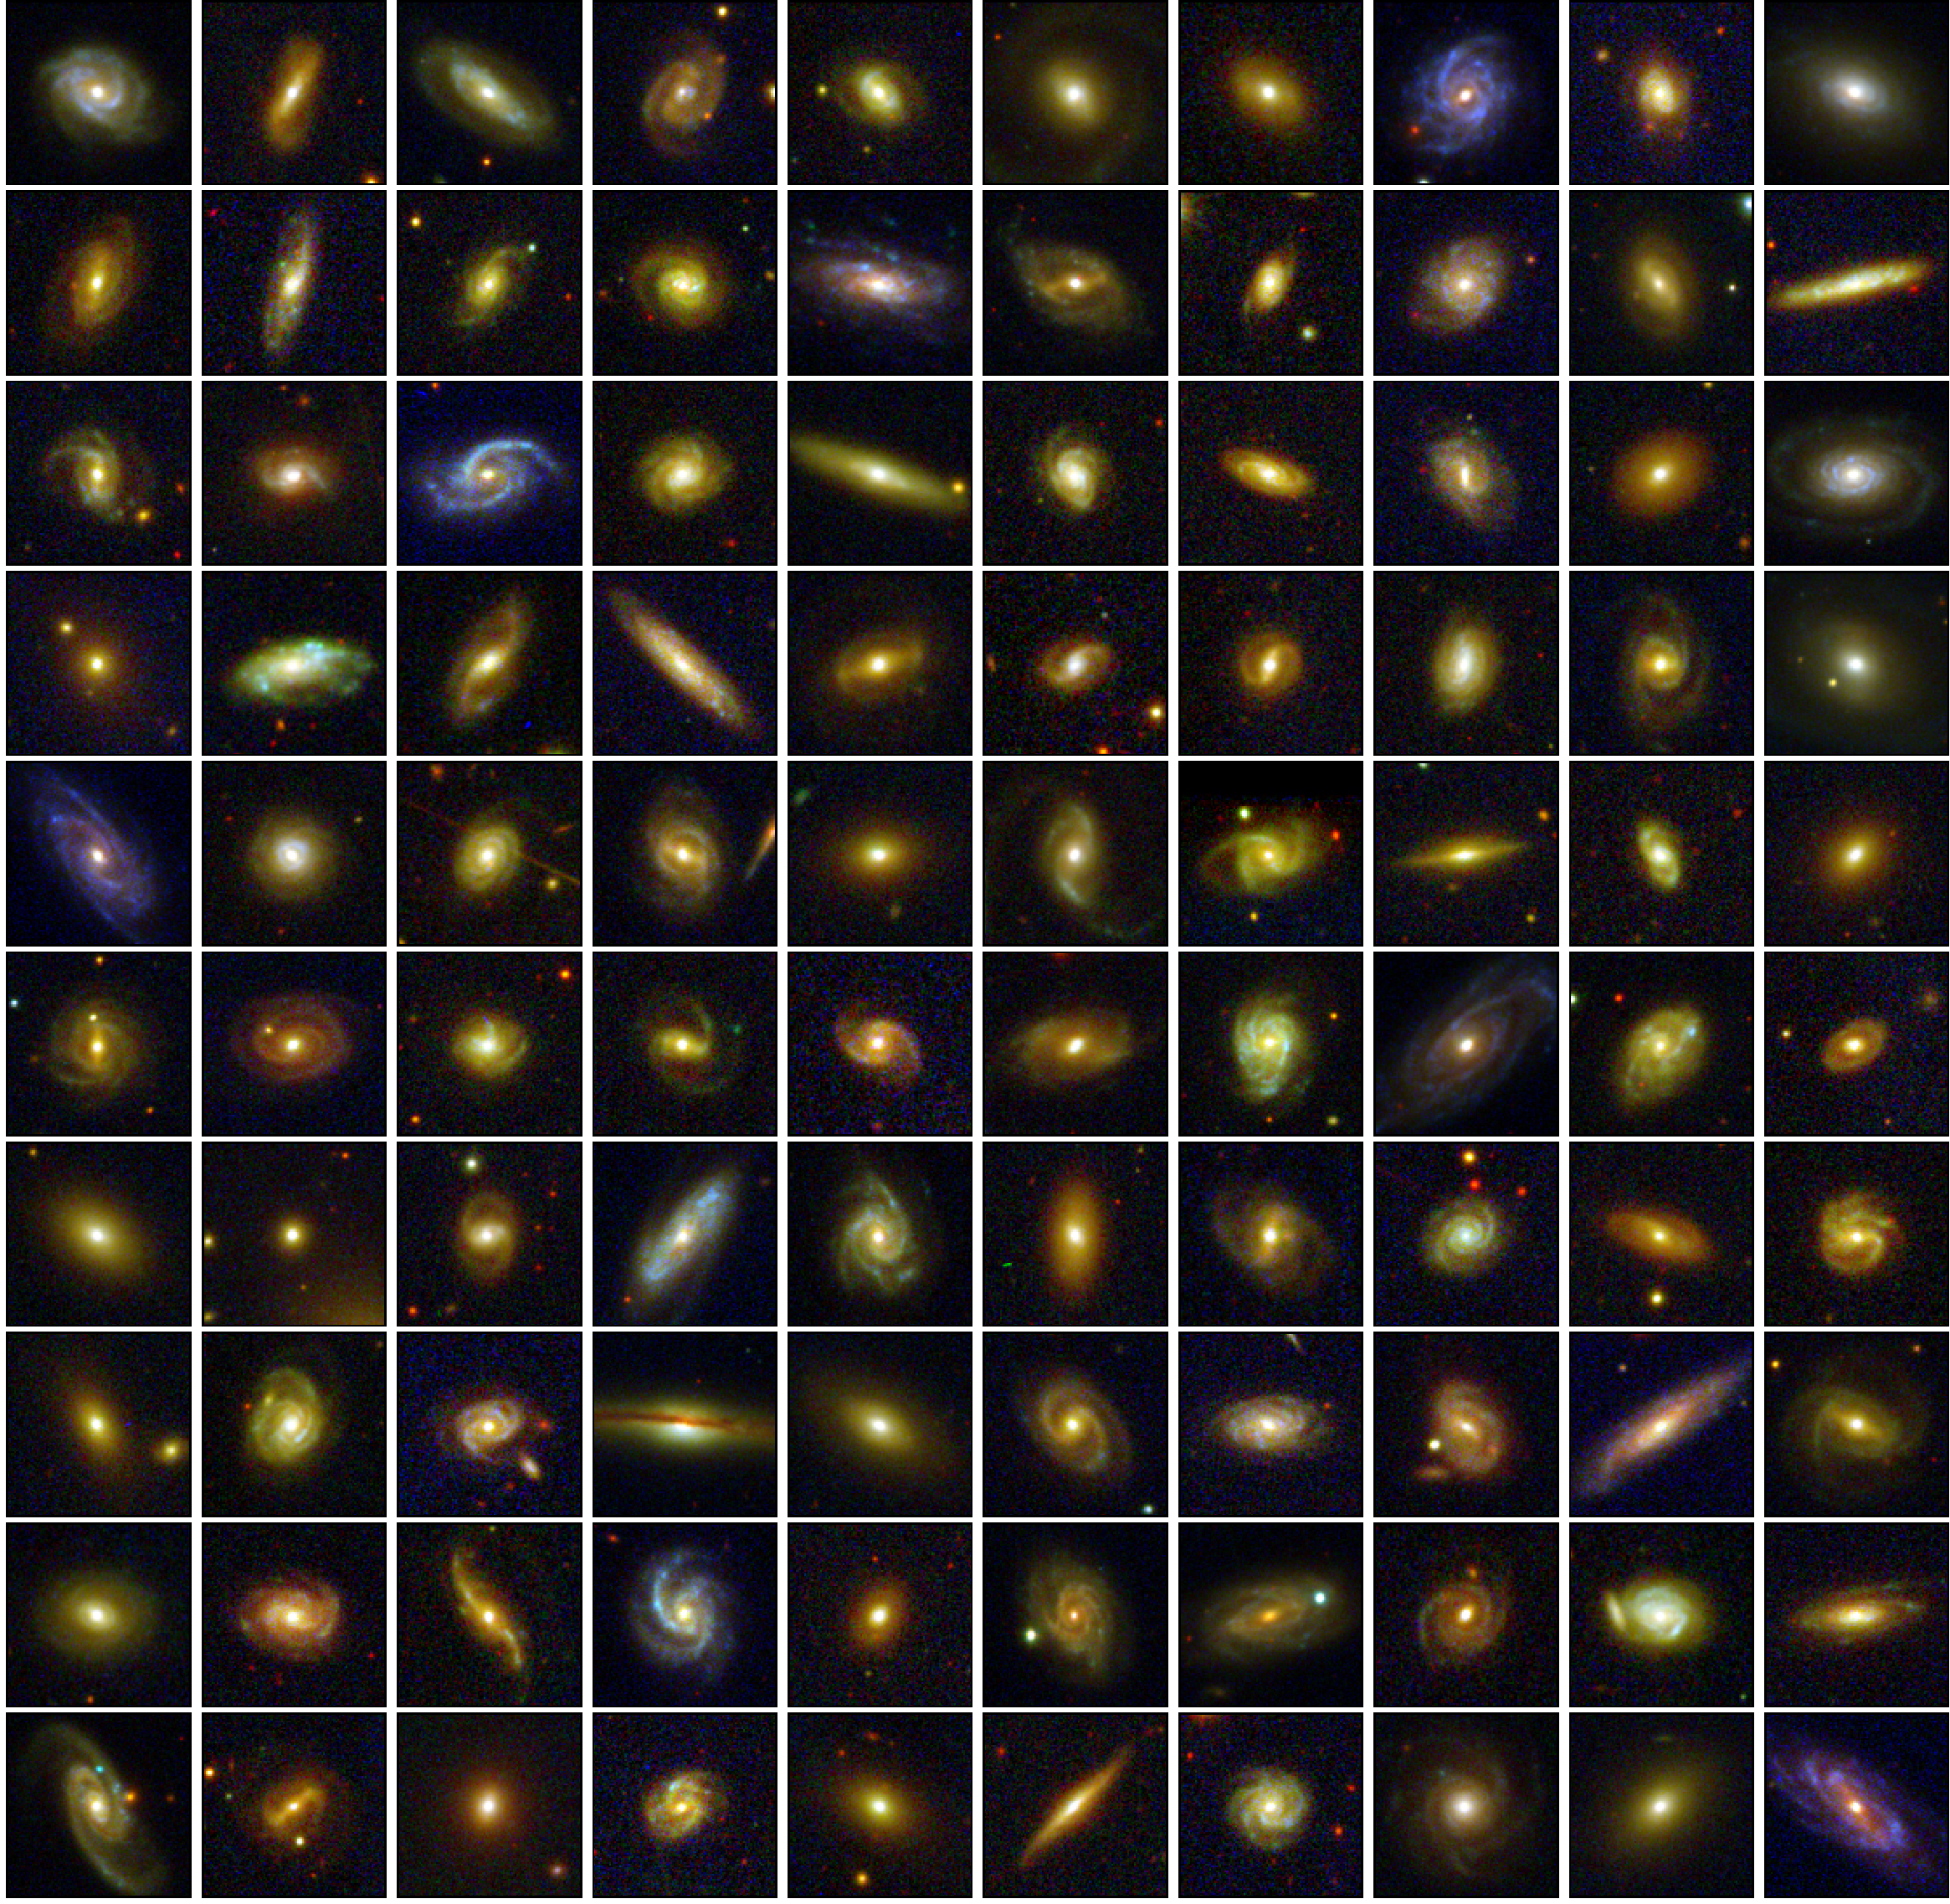
\includegraphics[width=\linewidth]{figures/galaxygrid_2}
  \caption{Exemplos de imagens de galáxias obtidas do S-PLUS e utilizadas nos conjuntos de treinamento, validação e teste, coloridas usando o método descrito na Seção \ref{section:preparacao}.}
  \label{fig:galaxy_grid}
\end{figure}


Para este trabalho queremos desenvolver uma técnica eficiente e automatizada para a  classificação morfológica de galáxias usando \emph{Deep Learning}. Para isso, primeiramente serão apresentados os dados utilizados e como os preparamos.

\subsection{Aquisição dos dados}

A imagem da galáxia, com sua respectiva classificação morfológica, é elemento crucial para se fazer o treinamento supervisionado de nossa Rede Neural Artificial. Para treinar a rede, de modo que esta aprenda a classificar galáxias através das imagens, é necessário fazê-la aprender as formas e padrões das galáxias. No nosso caso, utilizamos uma grande amostra de imagens de galáxias já classificadas visualmente por humanos.

Os dados aqui utilizados são as imagens das galáxias do levantamento S-PLUS e as classificações morfológicas do GalaxyZoo, que separam as galáxias entre espiral e elíptica. A associação destes dois conjuntos de dados é feita pela correlação das coordenadas do objeto no espaço. Ademais, apenas galáxias no S-PLUS com magnitudes $r_{auto}$ menores que 17 foram utilizadas. O valor de $r_{auto}$, que é dado em uma das colunas do catálogo do S-PLUS, representa aproximadamente o fluxo total de uma dada galáxia.  As imagens do S-PLUS foram obtidas através do banco de dados do projeto\footnote{\url{https://splus.cloud}}. A Figura \ref{fig:galaxy_grid} mostra exemplos d imagens RGB do S-PLUS utilizadas neste trabalho.

%%%%%%%%%%%%%%%%%%%%%%%%%%%%%%%%%%%%%%%%%%%
%% DIVISÃO DO CONJUNTO DE DADOS
%%%%%%%%%%%%%%%%%%%%%%%%%%%%%%%%%%%%%%%%%%%
\subsection{Divisão do conjunto de dados}
\label{section:divisao_conjunto_de_dados}

Todos os modelos usam os mesmos subconjuntos de dados para garantir que o desempenho de classificação do modelo não seja enviesado pela escolha dos lotes.

A distribuição de galáxias para cada subconjunto foi de 81\% para treinamento, 9\% para validação e 10\% para teste. A proporção de galáxias elípticas e espirais entre os subconjutos de treinamento, validação e teste é a mesma. Os conjuntos são constituídos por, aproximadamente, 68\% de galáxias espirais e 32\% de galáxias elípticas. O conjunto de treinamento é constituído por 2231 objetos, o conjunto de validação contém 248 objetos e o conjunto de teste contém 276 objetos, totalizando 2757 objetos no conjunto de dados.


\subsection{Comparação dos conjuntos de dados}

\begin{figure}[!ht]
  \centering
  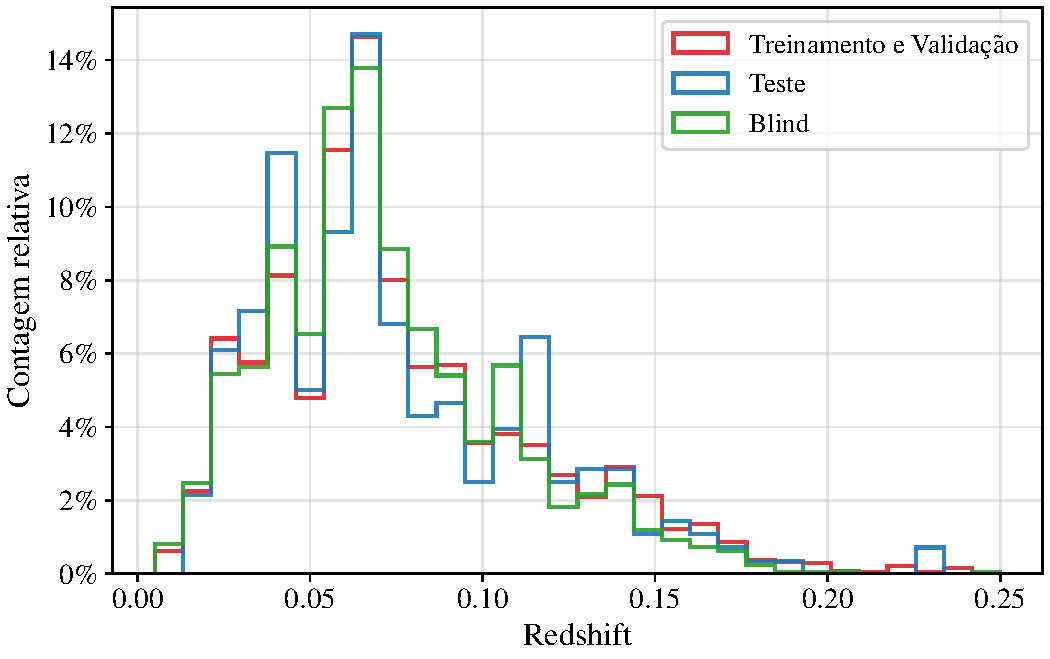
\includegraphics[width=0.58\linewidth]{figures/hist_170_redshift.pdf}
  \caption{Histograma com a contagem relativa da distribuição dos valores de \emph{redshift} das galáxias nos conjuntos de treinamento, validação, teste e \emph{blind}.}
  \label{fig:redshift-17}
\end{figure}

\begin{figure}[!ht]
  \centering
  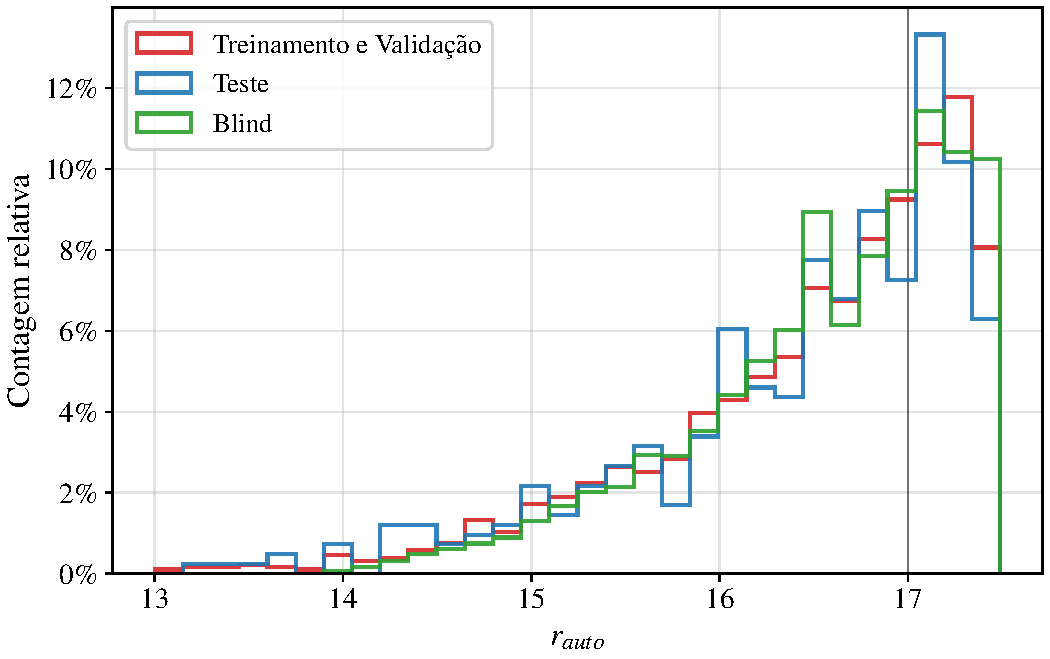
\includegraphics[width=0.58\linewidth]{figures/hist_rauto.pdf}
  \caption{Histograma com a contagem relativa da distribuição dos valores de $r_{auto}$ das galáxias nos conjuntos de treinamento, validação, teste e \emph{blind}.}
  \label{fig:dist-rauto}
\end{figure}

Para o desenvolvimento do trabalho, dividimos as amostras em subconjuntos distintos, com o objetivo final de fazer uma classificação de galáxias elípticas e espirais numa amostra ainda não classificada, denominada amostra \emph{blind}. Nesta seção, mostramos que as amostras de galáxias utilizadas nos conjuntos de treinamento, validação, teste e \emph{blind} têm distribuições equilibradas de medidas de brilho, determinadas através das magnitudes na banda r (que é a banda com maior sinal/ruído) e redshifts (desvios para o vermelho, que são proporcionais às distâncias dos objetos). Isto é importante para que a comparação dos diagramas cor-cor que serão mostrados na Figura \ref{fig:color-color}, na Seção \ref{section:resultados} faça sentido. A Figura \ref{fig:dist-rauto} mostra o histograma de magnitude das galáxias para valores de $r_{auto}$ entre 13 e 17. A Figura \ref{fig:redshift-17} mostra a distribuição de redshift para cada  conjunto.

\subsection{Conjunto de dados desbalanceado}

Como visto na Seção \ref{section:divisao_conjunto_de_dados}, aproximadamente 68\% das galáxias do conjunto de dados são espirais. Contudo, o desempenho dos algorítmos de \emph{machine learning} são afetados negativamente pela quantidade desproporcional de objetos entres as classes. Algumas técnicas testadas para melhorar o desempenho da rede são descritas a seguir.

\subsubsection{Subamostragem aleatória}

A subamostragem aleatória, \emph{random undersampling}, é a retirada aleatória de objetos do conjunto de trainamento pertencentes à classe com maior quantidade de elementos até que a proporção de objetos entre as classes fique equilibrada ($\approx 1:1$).

\subsubsection{Sobreamostragem aleatória}
Ao contrário da subamostragem, a sobreamostragem aleatória, \emph{random oversampling}, é a replicação de elementos da classe em minoria até que a proproção de objetos entre as classes fique equilibrada.

\subsubsection{Ponderamento das classes}
Ao contrário das técnicas anteriores, o ponderamento das classes (\emph{class weight}) não é uma técnica de reamostragem. Ela consiste na atribuição de pesos a cada classe, proporcionais a sua quantidade de elementos.
O peso $w_i$ da i-ésima classe tem o valor dado pela equação \eqref{eq:pesos}, baseada na heurística apresentada em \cite{KinZen01}.
\begin{equation}
  w_i = \frac{Q}{N \times C_i}
  \label{eq:pesos}
\end{equation}
onde, $Q$ é a quantidade total de objetos, $N$ é o número de classes e $C_i$ é o número de objetos da i-ésima classe.
